\hypertarget{a00001}{
\section{Dokumentacja klasy Baza}
\label{d8/d84/a00001}\index{Baza@{Baza}}
}
{\tt \#include $<$baza.hpp$>$}

\subsection*{Metody publiczne}
\begin{CompactItemize}
\item 
std::string \hyperlink{a00001_a09b37e4665bd7b2f2b8b54f8120f5be}{get\_\-passwd} (std::string login)
\begin{CompactList}\small\item\em Pobiera hasło uzytkownika z bazy. \item\end{CompactList}\item 
\hyperlink{a00001_8edd83a7fa98b203a1ab58157a1660a4}{Baza} ()
\begin{CompactList}\small\item\em Konstruktor pusty. \item\end{CompactList}\item 
void \hyperlink{a00001_bef61cc396e46d347a47c75e9ef8dfde}{connect} (const char $\ast$server, const char $\ast$login, const char $\ast$pass, const char $\ast$db)
\begin{CompactList}\small\item\em Łaczy się z bazą damych. \item\end{CompactList}\item 
mysqlpp::StoreQueryResult \hyperlink{a00001_02db3388d088212bd443ee39998b5cf8}{getFilesList} (int user\_\-id)
\begin{CompactList}\small\item\em Pobiera listę plików z bazy na podstawie ID uzytkownika. \item\end{CompactList}\item 
mysqlpp::StoreQueryResult \hyperlink{a00001_2eace36725672b3a4ce639f91fe7d9bd}{getFilesList} (std::string user)
\begin{CompactList}\small\item\em Najpierw wywołuje \hyperlink{a00001_65054f08c8fd7c600f6c2fe2c7f61a43}{getUserId()} potem z id otrzymanym z tamtąd wywołuje \hyperlink{a00001_02db3388d088212bd443ee39998b5cf8}{getFilesList(int user\_\-id)};. \item\end{CompactList}\item 
mysqlpp::StoreQueryResult \hyperlink{a00001_e4a033a65cb585aa91c15fd8b8fde764}{getFileInfo} (std::string file, std::string user)
\begin{CompactList}\small\item\em Podobnie jak getFilesList tylko ze pobiera informację o jednym pliku. \item\end{CompactList}\item 
mysqlpp::StoreQueryResult \hyperlink{a00001_1d1cfca062ab3117b2b97281df012823}{getFileInfo} (std::string file, int user\_\-id)
\item 
int \hyperlink{a00001_65054f08c8fd7c600f6c2fe2c7f61a43}{getUserId} (std::string user)
\begin{CompactList}\small\item\em Pobiera id uzytkownika 'user'. \item\end{CompactList}\item 
char \hyperlink{a00001_71ac41633bfb8e4b854aaa8281aac24c}{firends} (std::string user1, std::string user2)
\item 
bool \hyperlink{a00001_abbda65be49dfb28b1a578d0383599fa}{addFile} (std::string nazwa, std::string konto, int wielkosc, std::string hash=\char`\"{}-1\char`\"{}, int prawa=-1, int data=-1)
\begin{CompactList}\small\item\em Dodaje plik do bazy danych. \item\end{CompactList}\item 
bool \hyperlink{a00001_7161c573401166cc5f7d98ae6f335b44}{rmFile} (std::string nazwa, std::string konto, std::string hash)
\end{CompactItemize}
\subsection*{Atrybuty prywatne}
\begin{CompactItemize}
\item 
mysqlpp::Connection \hyperlink{a00001_f966364deec225fdf2d2d22550c71c88}{conn}
\begin{CompactList}\small\item\em Klasa do łączenia się z bazą danych. \item\end{CompactList}\end{CompactItemize}


\subsection{Opis szczegółowy}


Definicja w linii 8 pliku baza.hpp.

\subsection{Dokumentacja konstruktora i destruktora}
\hypertarget{a00001_8edd83a7fa98b203a1ab58157a1660a4}{
\index{Baza@{Baza}!Baza@{Baza}}
\index{Baza@{Baza}!Baza@{Baza}}
\subsubsection[{Baza}]{\setlength{\rightskip}{0pt plus 5cm}Baza::Baza ()\hspace{0.3cm}{\tt  \mbox{[}inline\mbox{]}}}}
\label{d8/d84/a00001_8edd83a7fa98b203a1ab58157a1660a4}


Konstruktor pusty. 



Definicja w linii 17 pliku baza.hpp.

\subsection{Dokumentacja funkcji składowych}
\hypertarget{a00001_abbda65be49dfb28b1a578d0383599fa}{
\index{Baza@{Baza}!addFile@{addFile}}
\index{addFile@{addFile}!Baza@{Baza}}
\subsubsection[{addFile}]{\setlength{\rightskip}{0pt plus 5cm}bool Baza::addFile (std::string {\em nazwa}, \/  std::string {\em konto}, \/  int {\em wielkosc}, \/  std::string {\em hash} = {\tt \char`\"{}-1\char`\"{}}, \/  int {\em prawa} = {\tt -1}, \/  int {\em data} = {\tt -1})}}
\label{d8/d84/a00001_abbda65be49dfb28b1a578d0383599fa}


Dodaje plik do bazy danych. 



Definicja w linii 239 pliku baza.cpp.

Oto graf wywołań dla tej funkcji:\nopagebreak
\begin{figure}[H]
\begin{center}
\leavevmode
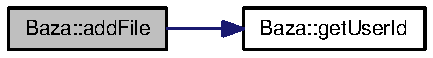
\includegraphics[width=122pt]{d8/d84/a00001_abbda65be49dfb28b1a578d0383599fa_cgraph}
\end{center}
\end{figure}
\hypertarget{a00001_bef61cc396e46d347a47c75e9ef8dfde}{
\index{Baza@{Baza}!connect@{connect}}
\index{connect@{connect}!Baza@{Baza}}
\subsubsection[{connect}]{\setlength{\rightskip}{0pt plus 5cm}void Baza::connect (const char $\ast$ {\em server}, \/  const char $\ast$ {\em login}, \/  const char $\ast$ {\em pass}, \/  const char $\ast$ {\em db})}}
\label{d8/d84/a00001_bef61cc396e46d347a47c75e9ef8dfde}


Łaczy się z bazą damych. 



I zamykamy połączenie 

Definicja w linii 3 pliku baza.cpp.

Here is the caller graph for this function:\nopagebreak
\begin{figure}[H]
\begin{center}
\leavevmode
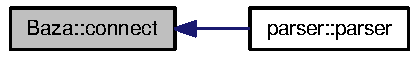
\includegraphics[width=118pt]{d8/d84/a00001_bef61cc396e46d347a47c75e9ef8dfde_icgraph}
\end{center}
\end{figure}
\hypertarget{a00001_71ac41633bfb8e4b854aaa8281aac24c}{
\index{Baza@{Baza}!firends@{firends}}
\index{firends@{firends}!Baza@{Baza}}
\subsubsection[{firends}]{\setlength{\rightskip}{0pt plus 5cm}char Baza::firends (std::string {\em user1}, \/  std::string {\em user2})}}
\label{d8/d84/a00001_71ac41633bfb8e4b854aaa8281aac24c}


Funkcja sprawdzająca czy użytkownicy są znajomymi \begin{Desc}
\item[Parametry:]
\begin{description}
\item[{\em user1}]Użytkownik pytający \item[{\em user2}]Użytkownik sprawdzany \end{description}
\end{Desc}
\begin{Desc}
\item[Zwraca:]char przedstawiający informację o rodzaju znajomości:$\backslash$ \end{Desc}
\hypertarget{a00001_a09b37e4665bd7b2f2b8b54f8120f5be}{
\index{Baza@{Baza}!get\_\-passwd@{get\_\-passwd}}
\index{get\_\-passwd@{get\_\-passwd}!Baza@{Baza}}
\subsubsection[{get\_\-passwd}]{\setlength{\rightskip}{0pt plus 5cm}std::string Baza::get\_\-passwd (std::string {\em login})}}
\label{d8/d84/a00001_a09b37e4665bd7b2f2b8b54f8120f5be}


Pobiera hasło uzytkownika z bazy. 



Definicja w linii 30 pliku baza.cpp.\hypertarget{a00001_1d1cfca062ab3117b2b97281df012823}{
\index{Baza@{Baza}!getFileInfo@{getFileInfo}}
\index{getFileInfo@{getFileInfo}!Baza@{Baza}}
\subsubsection[{getFileInfo}]{\setlength{\rightskip}{0pt plus 5cm}mysqlpp::StoreQueryResult Baza::getFileInfo (std::string {\em file}, \/  int {\em user\_\-id})}}
\label{d8/d84/a00001_1d1cfca062ab3117b2b97281df012823}




Definicja w linii 201 pliku baza.cpp.\hypertarget{a00001_e4a033a65cb585aa91c15fd8b8fde764}{
\index{Baza@{Baza}!getFileInfo@{getFileInfo}}
\index{getFileInfo@{getFileInfo}!Baza@{Baza}}
\subsubsection[{getFileInfo}]{\setlength{\rightskip}{0pt plus 5cm}mysqlpp::StoreQueryResult Baza::getFileInfo (std::string {\em file}, \/  std::string {\em user})}}
\label{d8/d84/a00001_e4a033a65cb585aa91c15fd8b8fde764}


Podobnie jak getFilesList tylko ze pobiera informację o jednym pliku. 



Definicja w linii 174 pliku baza.cpp.

Oto graf wywołań dla tej funkcji:\nopagebreak
\begin{figure}[H]
\begin{center}
\leavevmode
\includegraphics[width=129pt]{d8/d84/a00001_e4a033a65cb585aa91c15fd8b8fde764_cgraph}
\end{center}
\end{figure}
\hypertarget{a00001_2eace36725672b3a4ce639f91fe7d9bd}{
\index{Baza@{Baza}!getFilesList@{getFilesList}}
\index{getFilesList@{getFilesList}!Baza@{Baza}}
\subsubsection[{getFilesList}]{\setlength{\rightskip}{0pt plus 5cm}mysqlpp::StoreQueryResult Baza::getFilesList (std::string {\em user})}}
\label{d8/d84/a00001_2eace36725672b3a4ce639f91fe7d9bd}


Najpierw wywołuje \hyperlink{a00001_65054f08c8fd7c600f6c2fe2c7f61a43}{getUserId()} potem z id otrzymanym z tamtąd wywołuje \hyperlink{a00001_02db3388d088212bd443ee39998b5cf8}{getFilesList(int user\_\-id)};. 

Zapytanie o listę plików uzytkownika o nazwie podanej w zmiennej user. 

Definicja w linii 97 pliku baza.cpp.

Oto graf wywołań dla tej funkcji:\nopagebreak
\begin{figure}[H]
\begin{center}
\leavevmode
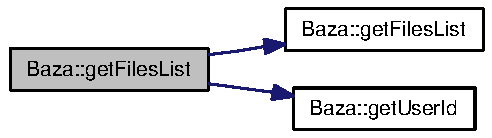
\includegraphics[width=136pt]{d8/d84/a00001_2eace36725672b3a4ce639f91fe7d9bd_cgraph}
\end{center}
\end{figure}
\hypertarget{a00001_02db3388d088212bd443ee39998b5cf8}{
\index{Baza@{Baza}!getFilesList@{getFilesList}}
\index{getFilesList@{getFilesList}!Baza@{Baza}}
\subsubsection[{getFilesList}]{\setlength{\rightskip}{0pt plus 5cm}mysqlpp::StoreQueryResult Baza::getFilesList (int {\em user\_\-id})}}
\label{d8/d84/a00001_02db3388d088212bd443ee39998b5cf8}


Pobiera listę plików z bazy na podstawie ID uzytkownika. 

Zapytanie o listę plikow uzytkownika po id uzytkownika z bazy accounts\_\-konto. 

Definicja w linii 61 pliku baza.cpp.

Here is the caller graph for this function:\nopagebreak
\begin{figure}[H]
\begin{center}
\leavevmode
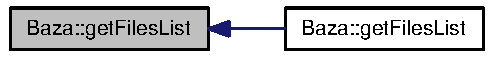
\includegraphics[width=136pt]{d8/d84/a00001_02db3388d088212bd443ee39998b5cf8_icgraph}
\end{center}
\end{figure}
\hypertarget{a00001_65054f08c8fd7c600f6c2fe2c7f61a43}{
\index{Baza@{Baza}!getUserId@{getUserId}}
\index{getUserId@{getUserId}!Baza@{Baza}}
\subsubsection[{getUserId}]{\setlength{\rightskip}{0pt plus 5cm}int Baza::getUserId (std::string {\em user})}}
\label{d8/d84/a00001_65054f08c8fd7c600f6c2fe2c7f61a43}


Pobiera id uzytkownika 'user'. 

Zapytanie o ID uzytkownika o loginie 'user' ale nie o id z auth\_\-user tylko o id z accounts\_\-konto. 

Definicja w linii 126 pliku baza.cpp.

Here is the caller graph for this function:\nopagebreak
\begin{figure}[H]
\begin{center}
\leavevmode
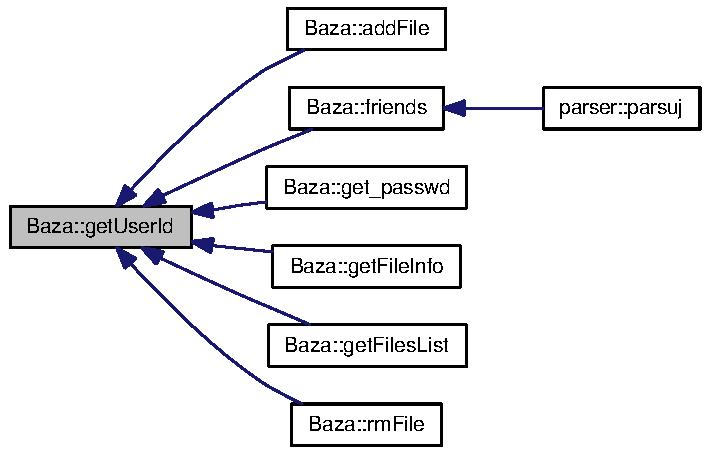
\includegraphics[width=132pt]{d8/d84/a00001_65054f08c8fd7c600f6c2fe2c7f61a43_icgraph}
\end{center}
\end{figure}
\hypertarget{a00001_7161c573401166cc5f7d98ae6f335b44}{
\index{Baza@{Baza}!rmFile@{rmFile}}
\index{rmFile@{rmFile}!Baza@{Baza}}
\subsubsection[{rmFile}]{\setlength{\rightskip}{0pt plus 5cm}bool Baza::rmFile (std::string {\em nazwa}, \/  std::string {\em konto}, \/  std::string {\em hash})}}
\label{d8/d84/a00001_7161c573401166cc5f7d98ae6f335b44}


Usuwa plik z bazy \begin{Desc}
\item[Parametry:]
\begin{description}
\item[{\em nazwa}]nazwa pliku do usuniecia \item[{\em konto}]nazwa konta z ktorego sie usuwa \item[{\em hash}]hash pliku (dla sprawdzenia czy napewno dobry plik) \end{description}
\end{Desc}
\begin{Desc}
\item[Zwraca:]czy operacja zakończona powodzeniem \end{Desc}


Definicja w linii 297 pliku baza.cpp.

Oto graf wywołań dla tej funkcji:\nopagebreak
\begin{figure}[H]
\begin{center}
\leavevmode
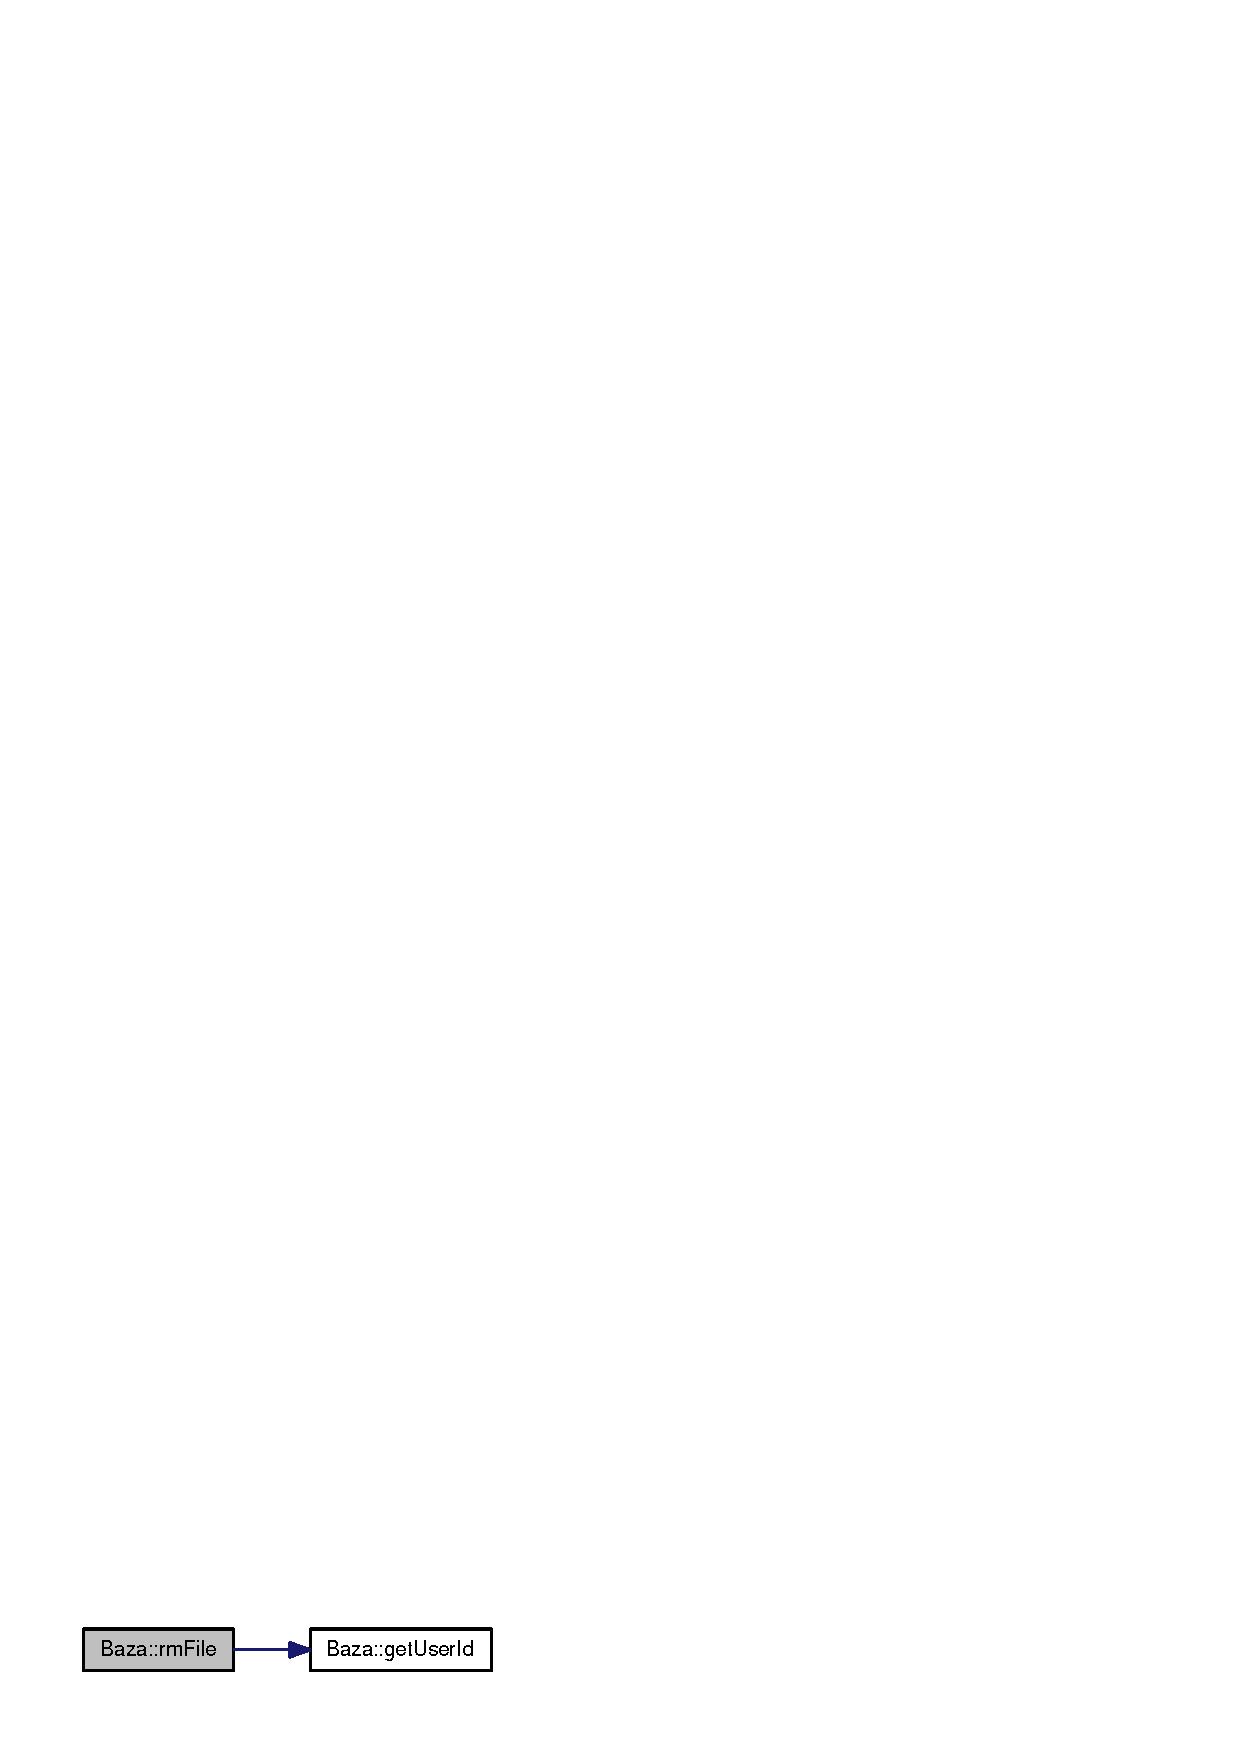
\includegraphics[width=120pt]{d8/d84/a00001_7161c573401166cc5f7d98ae6f335b44_cgraph}
\end{center}
\end{figure}


\subsection{Dokumentacja atrybutów składowych}
\hypertarget{a00001_f966364deec225fdf2d2d22550c71c88}{
\index{Baza@{Baza}!conn@{conn}}
\index{conn@{conn}!Baza@{Baza}}
\subsubsection[{conn}]{\setlength{\rightskip}{0pt plus 5cm}mysqlpp::Connection {\bf Baza::conn}\hspace{0.3cm}{\tt  \mbox{[}private\mbox{]}}}}
\label{d8/d84/a00001_f966364deec225fdf2d2d22550c71c88}


Klasa do łączenia się z bazą danych. 



Definicja w linii 12 pliku baza.hpp.

Dokumentacja dla tej klasy została wygenerowana z plików:\begin{CompactItemize}
\item 
/home/pawel/Dokumenty/Uczelnia/grupappz/Source/Ass8-server/\hyperlink{a00007}{baza.hpp}\item 
/home/pawel/Dokumenty/Uczelnia/grupappz/Source/Ass8-server/\hyperlink{a00006}{baza.cpp}\end{CompactItemize}
